
%
% 6.869 problem set 5
%
\documentclass[12pt,twoside]{article}

\usepackage{amsmath}
\usepackage{amssymb}
\usepackage{color}
\usepackage{clrscode}
\usepackage[pdftex]{graphicx}

% Cross-references for handout numbers.

% Updated to include SMA course for Fall 2001 -- cel

\newcommand{\name}{}


\usepackage{latexsym}
%\usepackage{bbm}
\usepackage{times,url}
\usepackage{clrscode}

\newcommand{\mitst}[1]{\begin{description}
\item[MIT students:] #1
\end{description}}
\newcommand{\smast}[1]{\begin{description}
\item[SMA students:] #1
\end{description}}

%\newcommand{\collabs}{Professors Srini Devadas, Nancy Lynch and Vinod Vaikuntanathan}
\newcommand{\subj}{6.006}

\newlength{\toppush}
\setlength{\toppush}{2\headheight}
\addtolength{\toppush}{\headsep}

\newcommand{\htitle}[2]{\noindent\vspace*{-\toppush}\newline\parbox{6.5in}
{\textit{6.869 Advances in Computer Vision}\hfill\name\newline
Andrew Moran \hfill #2\newline
\collabs\hfill #1 \vspace*{-.5ex}\newline
\mbox{}\hrulefill\mbox{}}\vspace*{1ex}\mbox{}\newline
\begin{center}{\Large\bf #1}\end{center}}

\newcommand{\handout}[2]{\thispagestyle{empty}
 \markboth{#1}{#1}
 \pagestyle{myheadings}\htitle{#1}{#2}}

\newcommand{\htitlewithouttitle}[2]{\noindent\vspace*{-\toppush}\newline\parbox{6.5in}
{\textit{Introduction to Algorithms}\hfill#2\newline
Massachusetts Institute of Technology \hfill 6.006\newline
%Singapore-MIT Alliance \hfill SMA5503\newline
\profs\hfill Handout #1\vspace*{-.5ex}\newline
\mbox{}\hrulefill\mbox{}}\vspace*{1ex}\mbox{}\newline}

\newcommand{\handoutwithouttitle}[2]{\thispagestyle{empty}
 \markboth{Handout \protect\ref{#1}}{Handout \protect\ref{#1}}
 \pagestyle{myheadings}\htitlewithouttitle{\protect\ref{#1}}{#2}}

\newcommand{\exam}[2]{% parameters: exam name, date
 \thispagestyle{empty}
 \markboth{\subj\ #1\hspace{1in}Name\hrulefill\ \ }%
          {\subj\ #1\hspace{1in}Name\hrulefill\ \ }
 \pagestyle{myheadings}\examtitle{#1}{#2}
 \renewcommand{\theproblem}{Problem \arabic{problemnum}}
}
\newcommand{\examsolutions}[3]{% parameters: handout, exam name, date
 \thispagestyle{empty}
 \markboth{Handout \protect\ref{#1}: #2}{Handout \protect\ref{#1}: #2}
% \pagestyle{myheadings}\htitle{\protect\ref{#1}}{#2}{#3}
 \pagestyle{myheadings}\examsolutionstitle{\protect\ref{#1}} {#2}{#3}
 \renewcommand{\theproblem}{Problem \arabic{problemnum}}
}
\newcommand{\examsolutionstitle}[3]{\noindent\vspace*{-\toppush}\newline\parbox{6.5in}
{\textit{Introduction to Algorithms}\hfill#3\newline
Massachusetts Institute of Technology \hfill 6.006\newline
%Singapore-MIT Alliance \hfill SMA5503\newline
\profs\hfill Handout #1\vspace*{-.5ex}\newline
\mbox{}\hrulefill\mbox{}}\vspace*{1ex}\mbox{}\newline
\begin{center}{\Large\bf #2}\end{center}}

\newcommand{\takehomeexam}[2]{% parameters: exam name, date
 \thispagestyle{empty}
 \markboth{\subj\ #1\hfill}{\subj\ #1\hfill}
 \pagestyle{myheadings}\examtitle{#1}{#2}
 \renewcommand{\theproblem}{Problem \arabic{problemnum}}
}

\makeatletter
\newcommand{\exambooklet}[2]{% parameters: exam name, date
 \thispagestyle{empty}
 \markboth{\subj\ #1}{\subj\ #1}
 \pagestyle{myheadings}\examtitle{#1}{#2}
 \renewcommand{\theproblem}{Problem \arabic{problemnum}}
 \renewcommand{\problem}{\newpage
 \item \let\@currentlabel=\theproblem
 \markboth{\subj\ #1, \theproblem}{\subj\ #1, \theproblem}}
}
\makeatother


\newcommand{\examtitle}[2]{\noindent\vspace*{-\toppush}\newline\parbox{6.5in}
{\textit{Introduction to Algorithms}\hfill#2\newline
Massachusetts Institute of Technology \hfill 6.006 Spring 2014\newline
%Singapore-MIT Alliance \hfill SMA5503\newline
\profs\hfill #1\vspace*{-.5ex}\newline
\mbox{}\hrulefill\mbox{}}\vspace*{1ex}\mbox{}\newline
\begin{center}{\Large\bf #1}\end{center}}

\newcommand{\grader}[1]{\hspace{1cm}\textsf{\textbf{#1}}\hspace{1cm}}

\newcommand{\points}[1]{[#1 points]\ }
\newcommand{\parts}[1]
{
  \ifnum#1=1
  (1 part)
  \else
  (#1 parts)
  \fi
  \ 
}

\newcommand{\bparts}{\begin{problemparts}}
\newcommand{\eparts}{\end{problemparts}}
\newcommand{\ppart}{\problempart}

%\newcommand{\lg} {lg\ }

\setlength{\oddsidemargin}{0pt}
\setlength{\evensidemargin}{0pt}
\setlength{\textwidth}{6.5in}
\setlength{\topmargin}{0in}
\setlength{\textheight}{8.5in}


\newcommand{\Spawn}{{\bf spawn} }
\newcommand{\Sync}{{\bf sync}}

\renewcommand{\cases}[1]{\left\{ \begin{array}{ll}#1\end{array}\right.}
\newcommand{\cif}[1]{\mbox{if $#1$}}
\newcommand{\cwhen}[1]{\mbox{when $#1$}}

\newcounter{problemnum}
\newcommand{\theproblem}{Problem \theproblemsetnum-\arabic{problemnum}}
\newenvironment{problems}{
        \begin{list}{{\bf \theproblem. \hspace*{0.5em}}}
        {\setlength{\leftmargin}{0em}
         \setlength{\rightmargin}{0em}
         \setlength{\labelwidth}{0em}
         \setlength{\labelsep}{0em}
         \usecounter{problemnum}}}{\end{list}}
\makeatletter
\newcommand{\problem}[1][{}]{\item \let\@currentlabel=\theproblem \textbf{#1}}
\makeatother

\newcounter{problempartnum}[problemnum]
\newenvironment{problemparts}{
        \begin{list}{{\bf (\alph{problempartnum})}}
        {\setlength{\leftmargin}{2.5em}
         \setlength{\rightmargin}{2.5em}
         \setlength{\labelsep}{0.5em}}}{\end{list}}
\newcommand{\problempart}{\addtocounter{problempartnum}{1}\item}

\newenvironment{truefalseproblemparts}{
        \begin{list}{{\bf (\alph{problempartnum})\ \ \ T\ \ F\hfil}}
        {\setlength{\leftmargin}{4.5em}
         \setlength{\rightmargin}{2.5em}
         \setlength{\labelsep}{0.5em}
         \setlength{\labelwidth}{4.5em}}}{\end{list}}

\newcounter{exercisenum}
\newcommand{\theexercise}{Exercise \theproblemsetnum-\arabic{exercisenum}}
\newenvironment{exercises}{
        \begin{list}{{\bf \theexercise. \hspace*{0.5em}}}
        {\setlength{\leftmargin}{0em}
         \setlength{\rightmargin}{0em}
         \setlength{\labelwidth}{0em}
         \setlength{\labelsep}{0em}
        \usecounter{exercisenum}}}{\end{list}}
\makeatletter
\newcommand{\exercise}{\item \let\@currentlabel=\theexercise}
\makeatother

\newcounter{exercisepartnum}[exercisenum]
%\newcommand{\problem}[1]{\medskip\mbox{}\newline\noindent{\bf Problem #1.}\hspace*{1em}}
%\newcommand{\exercise}[1]{\medskip\mbox{}\newline\noindent{\bf Exercise #1.}\hspace*{1em}}

\newenvironment{exerciseparts}{
        \begin{list}{{\bf (\alph{exercisepartnum})}}
        {\setlength{\leftmargin}{2.5em}
         \setlength{\rightmargin}{2.5em}
         \setlength{\labelsep}{0.5em}}}{\end{list}}
\newcommand{\exercisepart}{\addtocounter{exercisepartnum}{1}\item}


% Macros to make captions print with small type and 'Figure xx' in bold.
\makeatletter
\def\fnum@figure{{\bf Figure \thefigure}}
\def\fnum@table{{\bf Table \thetable}}
\let\@mycaption\caption
%\long\def\@mycaption#1[#2]#3{\addcontentsline{\csname
%  ext@#1\endcsname}{#1}{\protect\numberline{\csname 
%  the#1\endcsname}{\ignorespaces #2}}\par
%  \begingroup
%    \@parboxrestore
%    \small
%    \@makecaption{\csname fnum@#1\endcsname}{\ignorespaces #3}\par
%  \endgroup}
%\def\mycaption{\refstepcounter\@captype \@dblarg{\@mycaption\@captype}}
%\makeatother
\let\mycaption\caption
%\newcommand{\figcaption}[1]{\mycaption[]{#1}}

\newcounter{totalcaptions}
\newcounter{totalart}

\newcommand{\figcaption}[1]{\addtocounter{totalcaptions}{1}\caption[]{#1}}

% \psfigures determines what to do for figures:
%       0 means just leave vertical space
%       1 means put a vertical rule and the figure name
%       2 means insert the PostScript version of the figure
%       3 means put the figure name flush left or right
\newcommand{\psfigures}{0}
\newcommand{\spacefigures}{\renewcommand{\psfigures}{0}}
\newcommand{\rulefigures}{\renewcommand{\psfigures}{1}}
\newcommand{\macfigures}{\renewcommand{\psfigures}{2}}
\newcommand{\namefigures}{\renewcommand{\psfigures}{3}}

\newcommand{\figpart}[1]{{\bf (#1)}\nolinebreak[2]\relax}
\newcommand{\figparts}[2]{{\bf (#1)--(#2)}\nolinebreak[2]\relax}


\macfigures     % STATE

% When calling \figspace, make sure to leave a blank line afterward!!
% \widefigspace is for figures that are more than 28pc wide.
\newlength{\halffigspace} \newlength{\wholefigspace}
\newlength{\figruleheight} \newlength{\figgap}
\newcommand{\setfiglengths}{\ifnum\psfigures=1\setlength{\figruleheight}{\hruleheight}\setlength{\figgap}{1em}\else\setlength{\figruleheight}{0pt}\setlength{\figgap}{0em}\fi}
\newcommand{\figspace}[2]{\ifnum\psfigures=0\leavefigspace{#1}\else%
\setfiglengths%
\setlength{\wholefigspace}{#1}\setlength{\halffigspace}{.5\wholefigspace}%
\rule[-\halffigspace]{\figruleheight}{\wholefigspace}\hspace{\figgap}#2\fi}
\newlength{\widefigspacewidth}
% Make \widefigspace put the figure flush right on the text page.
\newcommand{\widefigspace}[2]{
\ifnum\psfigures=0\leavefigspace{#1}\else%
\setfiglengths%
\setlength{\widefigspacewidth}{28pc}%
\addtolength{\widefigspacewidth}{-\figruleheight}%
\setlength{\wholefigspace}{#1}\setlength{\halffigspace}{.5\wholefigspace}%
\makebox[\widefigspacewidth][r]{#2\hspace{\figgap}}\rule[-\halffigspace]{\figruleheight}{\wholefigspace}\fi}
\newcommand{\leavefigspace}[1]{\setlength{\wholefigspace}{#1}\setlength{\halffigspace}{.5\wholefigspace}\rule[-\halffigspace]{0em}{\wholefigspace}}

% Commands for including figures with macpsfig.
% To use these commands, documentstyle ``macpsfig'' must be specified.
\newlength{\macfigfill}
\makeatother
\newlength{\bbx}
\newlength{\bby}
\newcommand{\macfigure}[5]{\addtocounter{totalart}{1}
\ifnum\psfigures=2%
\setlength{\bbx}{#2}\addtolength{\bbx}{#4}%
\setlength{\bby}{#3}\addtolength{\bby}{#5}%
\begin{flushleft}
\ifdim#4>28pc\setlength{\macfigfill}{#4}\addtolength{\macfigfill}{-28pc}\hspace*{-\macfigfill}\fi%
\mbox{\psfig{figure=./#1.ps,%
bbllx=#2,bblly=#3,bburx=\bbx,bbury=\bby}}
\end{flushleft}%
\else\ifdim#4>28pc\widefigspace{#5}{#1}\else\figspace{#5}{#1}\fi\fi}
\makeatletter

\newlength{\savearraycolsep}
\newcommand{\narrowarray}[1]{\setlength{\savearraycolsep}{\arraycolsep}\setlength{\arraycolsep}{#1\arraycolsep}}
\newcommand{\normalarray}{\setlength{\arraycolsep}{\savearraycolsep}}

\newcommand{\hint}{{\em Hint:\ }}

% Macros from /th/u/clr/mac.tex

\newcommand{\set}[1]{\left\{ #1 \right\}}
\newcommand{\abs}[1]{\left| #1\right|}
\newcommand{\card}[1]{\left| #1\right|}
\newcommand{\floor}[1]{\left\lfloor #1 \right\rfloor}
\newcommand{\ceil}[1]{\left\lceil #1 \right\rceil}
\newcommand{\ang}[1]{\ifmmode{\left\langle #1 \right\rangle}
   \else{$\left\langle${#1}$\right\rangle$}\fi}
        % the \if allows use outside mathmode,
        % but will swallow following space there!
\newcommand{\paren}[1]{\left( #1 \right)}
\newcommand{\bracket}[1]{\left[ #1 \right]}
\newcommand{\prob}[1]{\Pr\left\{ #1 \right\}}
\newcommand{\Var}{\mathop{\rm Var}\nolimits}
\newcommand{\expect}[1]{{\rm E}\left[ #1 \right]}
\newcommand{\expectsq}[1]{{\rm E}^2\left[ #1 \right]}
\newcommand{\variance}[1]{{\rm Var}\left[ #1 \right]}
\renewcommand{\choose}[2]{{{#1}\atopwithdelims(){#2}}}
\def\pmod#1{\allowbreak\mkern12mu({\rm mod}\,\,#1)}
\newcommand{\matx}[2]{\left(\begin{array}{*{#1}{c}}#2\end{array}\right)}
\newcommand{\Adj}{\mathop{\rm Adj}\nolimits}

\newtheorem{theorem}{Theorem}
\newtheorem{lemma}[theorem]{Lemma}
\newtheorem{corollary}[theorem]{Corollary}
\newtheorem{xample}{Example}
\newtheorem{definition}{Definition}
\newenvironment{example}{\begin{xample}\rm}{\end{xample}}
\newcommand{\proof}{\noindent{\em Proof.}\hspace{1em}}
\def\squarebox#1{\hbox to #1{\hfill\vbox to #1{\vfill}}}
\newcommand{\qedbox}{\vbox{\hrule\hbox{\vrule\squarebox{.667em}\vrule}\hrule}}
\newcommand{\qed}{\nopagebreak\mbox{}\hfill\qedbox\smallskip}
\newcommand{\eqnref}[1]{(\protect\ref{#1})}

%%\newcommand{\twodots}{\mathinner{\ldotp\ldotp}}
\newcommand{\transpose}{^{\mbox{\scriptsize \sf T}}}
\newcommand{\amortized}[1]{\widehat{#1}}

\newcommand{\punt}[1]{}

%%% command for putting definitions into boldface
% New style for defined terms, as of 2/23/88, redefined by THC.
\newcommand{\defn}[1]{{\boldmath\textit{\textbf{#1}}}}
\newcommand{\defi}[1]{{\textit{\textbf{#1\/}}}}

\newcommand{\red}{\leq_{\rm P}}
\newcommand{\lang}[1]{%
\ifmmode\mathord{\mathcode`-="702D\rm#1\mathcode`\-="2200}\else{\rm#1}\fi}

%\newcommand{\ckt}[1]{\ifmmode\mathord{\mathcode`-="702D\sc #1\mathcode`\-="2200}\else$\mathord{\mathcode`-="702D\sc #1\mathcode`\-="2200}$\fi}
\newcommand{\ckt}[1]{\ifmmode \sc #1\else$\sc #1$\fi}

%% Margin notes - use \notesfalse to turn off notes.
\setlength{\marginparwidth}{0.6in}
\reversemarginpar
\newif\ifnotes
\notestrue
\newcommand{\longnote}[1]{
  \ifnotes
    {\medskip\noindent Note: \marginpar[\hfill$\Longrightarrow$]
      {$\Longleftarrow$}{#1}\medskip}
  \fi}
\newcommand{\note}[1]{
  \ifnotes
    {\marginpar{\tiny \raggedright{#1}}}
  \fi}


\newcommand{\reals}{\mathbbm{R}}
\newcommand{\integers}{\mathbbm{Z}}
\newcommand{\naturals}{\mathbbm{N}}
\newcommand{\rationals}{\mathbbm{Q}}
\newcommand{\complex}{\mathbbm{C}}

\newcommand{\oldreals}{{\bf R}}
\newcommand{\oldintegers}{{\bf Z}}
\newcommand{\oldnaturals}{{\bf N}}
\newcommand{\oldrationals}{{\bf Q}}
\newcommand{\oldcomplex}{{\bf C}}

\newcommand{\w}{\omega}                 %% for fft chapter

\newenvironment{closeitemize}{\begin{list}
{$\bullet$}
{\setlength{\itemsep}{-0.2\baselineskip}
\setlength{\topsep}{0.2\baselineskip}
\setlength{\parskip}{0pt}}}
{\end{list}}

% These are necessary within a {problems} environment in order to restore
% the default separation between bullets and items.
\newenvironment{normalitemize}{\setlength{\labelsep}{0.5em}\begin{itemize}}
                              {\end{itemize}}
\newenvironment{normalenumerate}{\setlength{\labelsep}{0.5em}\begin{enumerate}}
                                {\end{enumerate}}

%\def\eqref#1{Equation~(\ref{eq:#1})}
%\newcommand{\eqref}[1]{Equation (\ref{eq:#1})}
\newcommand{\eqreftwo}[2]{Equations (\ref{eq:#1}) and~(\ref{eq:#2})}
\newcommand{\ineqref}[1]{Inequality~(\ref{ineq:#1})}
\newcommand{\ineqreftwo}[2]{Inequalities (\ref{ineq:#1}) and~(\ref{ineq:#2})}

\newcommand{\figref}[1]{Figure~\ref{fig:#1}}
\newcommand{\figreftwo}[2]{Figures \ref{fig:#1} and~\ref{fig:#2}}

\newcommand{\liref}[1]{line~\ref{li:#1}}
\newcommand{\Liref}[1]{Line~\ref{li:#1}}
\newcommand{\lirefs}[2]{lines \ref{li:#1}--\ref{li:#2}}
\newcommand{\Lirefs}[2]{Lines \ref{li:#1}--\ref{li:#2}}
\newcommand{\lireftwo}[2]{lines \ref{li:#1} and~\ref{li:#2}}
\newcommand{\lirefthree}[3]{lines \ref{li:#1}, \ref{li:#2}, and~\ref{li:#3}}

\newcommand{\lemlabel}[1]{\label{lem:#1}}
\newcommand{\lemref}[1]{Lemma~\ref{lem:#1}} 

\newcommand{\exref}[1]{Exercise~\ref{ex:#1}}

\newcommand{\handref}[1]{Handout~\ref{#1}}

\newcommand{\defref}[1]{Definition~\ref{def:#1}}

% (1997.8.16: Victor Luchangco)
% Modified \hlabel to only get date and to use handouts counter for number.
%   New \handout and \handoutwithouttitle commands in newmac.tex use this.
%   The date is referenced by <label>-date.
%   (Retained old definition as \hlabelold.)
%   Defined \hforcelabel to use an argument instead of the handouts counter.

\newcounter{handouts}
\setcounter{handouts}{0}

\newcommand{\hlabel}[2]{%
\stepcounter{handouts}
{\edef\next{\write\@auxout{\string\newlabel{#1}{{\arabic{handouts}}{0}}}}\next}
\write\@auxout{\string\newlabel{#1-date}{{#2}{0}}}
}

\newcommand{\hforcelabel}[3]{%          Does not step handouts counter.
\write\@auxout{\string\newlabel{#1}{{#2}{0}}}
\write\@auxout{\string\newlabel{#1-date}{{#3}{0}}}}


% less ugly underscore
% --juang, 2008 oct 05
\renewcommand{\_}{\vrule height 0 pt depth 0.4 pt width 0.5 em \,}


\setlength{\oddsidemargin}{0pt}
\setlength{\evensidemargin}{0pt}
\setlength{\textwidth}{6.5in}
\setlength{\topmargin}{0in}
\setlength{\textheight}{8.5in}

\newcommand{\theproblemsetnum}{5}
\newcommand{\partaduedate}{Oct 9, 2014 (1:00pm)}
\newcommand{\collabs}{Collaborators: None}
\newcommand{\tabUnit}{3ex}
\newcommand{\tabT}{\hspace*{\tabUnit}}

\title{6.869 PSET 5}

\begin{document}

\handout{Problem Set \theproblemsetnum}{Oct 9, 2014 (1:00pm)}
\tabT Resources with corresponding images and code are on Stellar under \texttt{andrewmo@mit.edu}.  The files are in the \texttt{pset5.zip} folder.  To reproduce the below figures, run \texttt{Prob1.m} and \texttt{pset5\_2main.m}.


\section*{Problem 5.1}
\tabT In this problem, I implemented the belief propagation algorithm for contstructing dense stereo correspondence.  This utilized disparities of up to L=10 pixels.  Below are the steps taken to achieve the desired results.

\textbf{(A)} The data term is represented as $\phi(x_{i}|y_{i}^{l}, y_{i}^{r}) \propto exp(-\lambda|y_{i}^{l} - y_{i-x_{i}}^{r}|)$
\newline
\tabT\tabT\tabT \textbf{Code:} \texttt{D(y,x,l) = exp(-lambda*abs(y\_l - y\_r));}
\newline

\textbf{(B)} The smoothness term is represented as $\psi(x_{i}, x_{i+1}) \propto exp(-|x_{i} - x_{i+1}|)$
\newline
\tabT\tabT\tabT \textbf{Code:} \texttt{P(l1,l2) = exp(-abs(dx1-dx2));}
\newline

\textbf{(C)} Below is the hidden Markov model used in this assignment.

\begin{center}
\DeclareGraphicsExtensions{.pdf,.png,.jpg}
    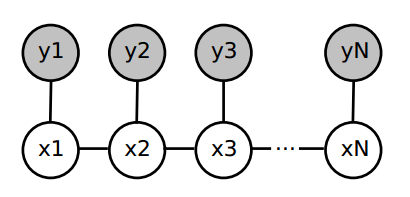
\includegraphics[scale=.5]{markov} 
\end{center}

The gray nodes are observed pixels, and the white nodes are the disparity that we wish to infer.  Messages from node j to node i were computed as follows: $m_{ji}(x_{i}) = \sum\limits_{x_{j}} \psi_{ij}(x_i, x_j) \prod\limits_{k \in \eta(j)/i} m_{kj}(x_j)$ 
\newline
It was key to note that the message from the observed state was the data term.  As a result, the generic form of calculting messages in code is shown below:
\newline
\tabT\tabT\tabT \textbf{Code:} \texttt{ P * [D(y,x,:) .* msgs\_sumprod(y,x,DIRECTION,:)]; }
\newline

\textbf{(D)} We cane find the marginal probability by using the messages computed earlier as follows:
\newline
\begin{center}
$p(x|y^l, y^r) = \frac{1}{Z} \prod\limits_{i=1}^{N} \phi(x_{i}|y_{i}^{l}, y_{i}^{r}) \psi(x_{i}, x_{i+1}) = \prod\limits_{j \in \eta{i}} m_{ji}(x_i)$
\end{center}

In summary, each marginal is computed using incoming messages from the top, left, and right neighboring nodes.
\newline

\textbf{(E)} Computing the mean was finding the expectation for each pixel using both the disparities and their marginal probabilities.  This was calculated as $\sum\limits_{l} lP(x_i = l)$.  
\newline

\textbf{(F)} Below are the plots for the marginals of the green and red pixel.  
\newline

\hspace{-70pt}
\DeclareGraphicsExtensions{.pdf,.png,.jpg}
    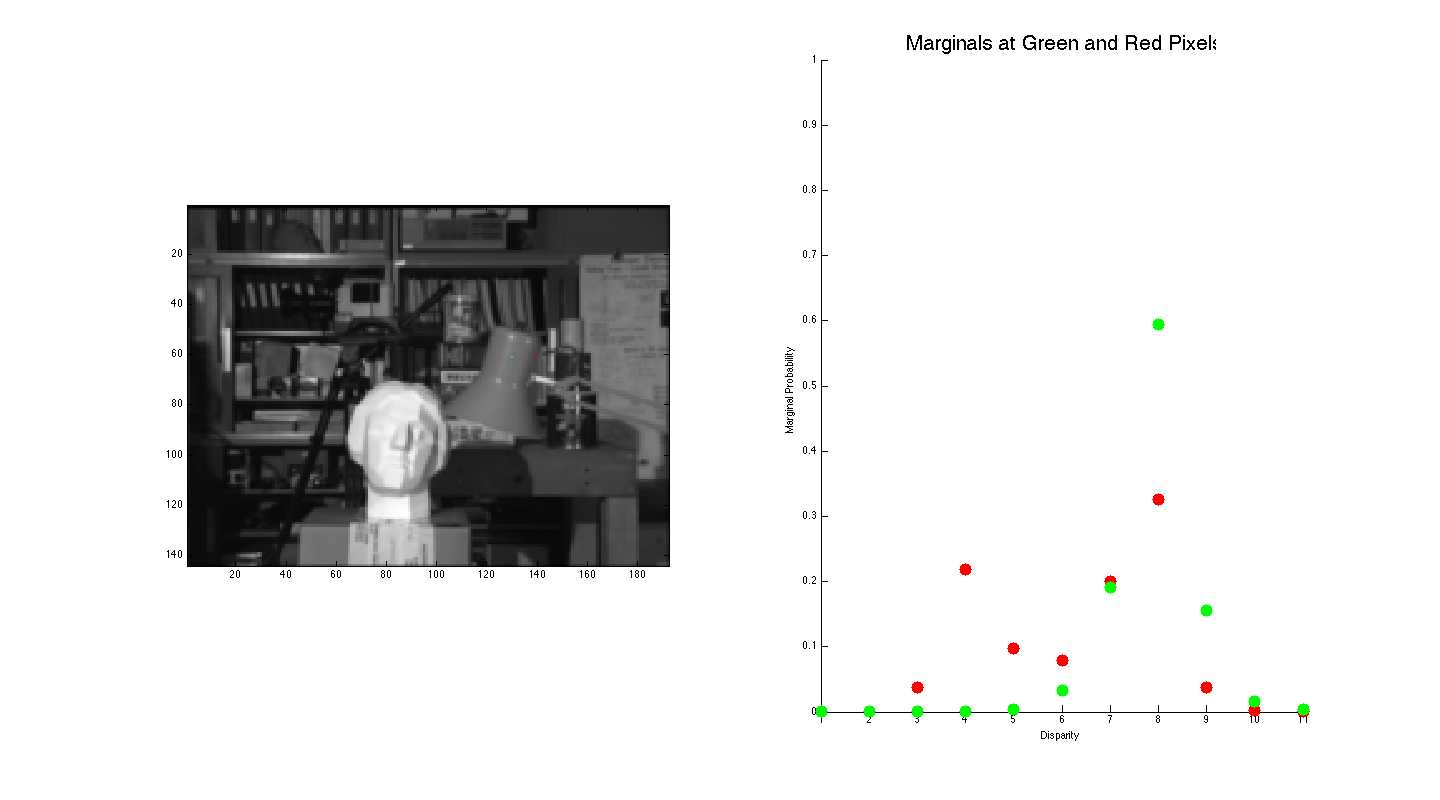
\includegraphics[scale=.4]{5_1d} 

The marginals at an edge pixel has very high probability since that's where the largest change in data occurs.  The green pixel is further from an edge, put when the disparity is large enough that it reaches an edge, the probability marginal has a significant spike at that point.  On the otherhand, the red pixel is on an edge.  Therefore small disparities either to the right or left of the pixel will show noticeable spikes in its left and right marginals (however, not as large).
\newline

\textbf{(G)} Mean and MAP estimates of the disparity for $\lambda = .2$ for scanline 61 (MAP explained in (j)):  
\newline 

\DeclareGraphicsExtensions{.pdf,.png,.jpg}
    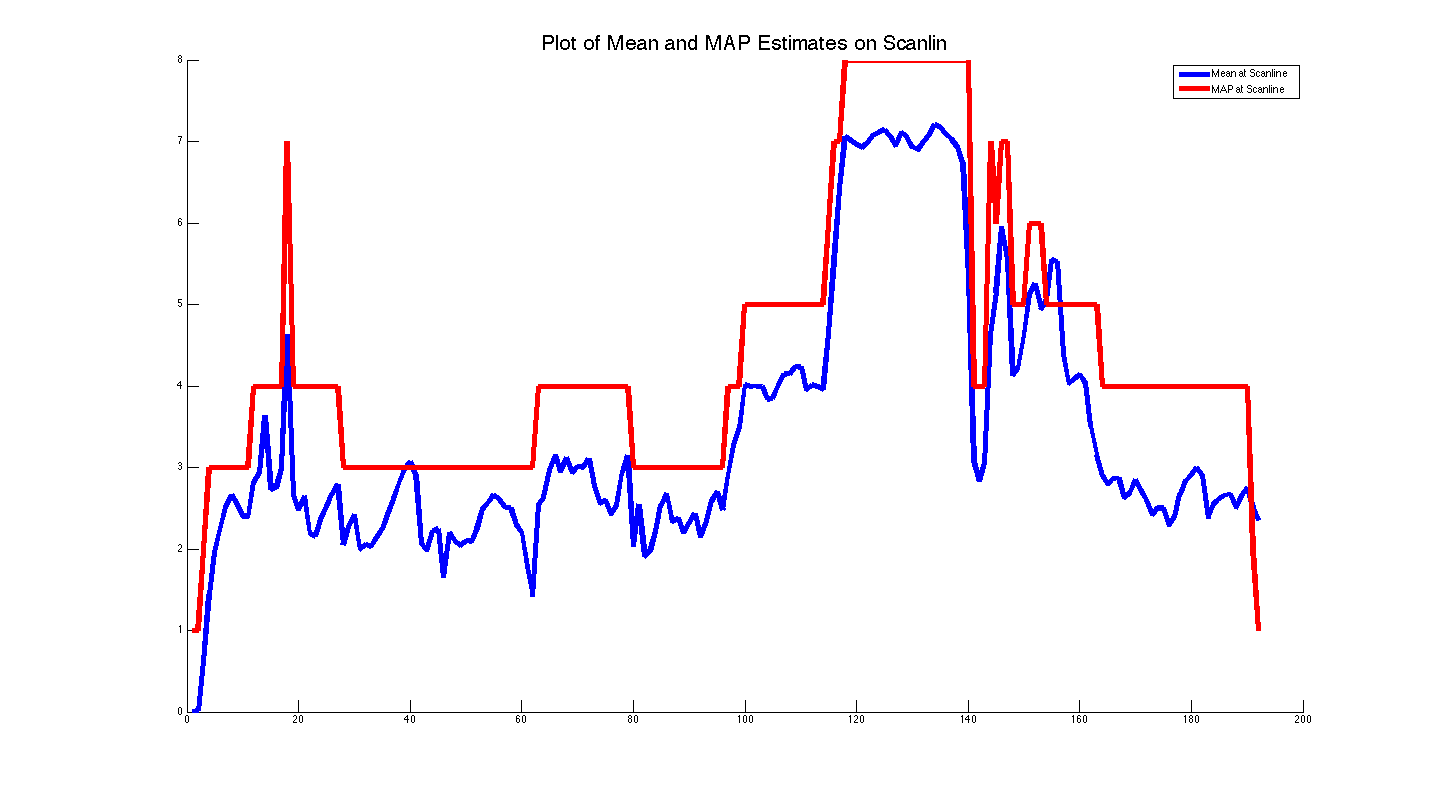
\includegraphics[scale=.3]{5_1e}

\textbf{(H)} Mean and MAP estimates of the disparity for $\lambda = 0,.1,.5,1$ respectively:  
\newline 


\DeclareGraphicsExtensions{.pdf,.png,.jpg}
	\hspace{-40pt}
    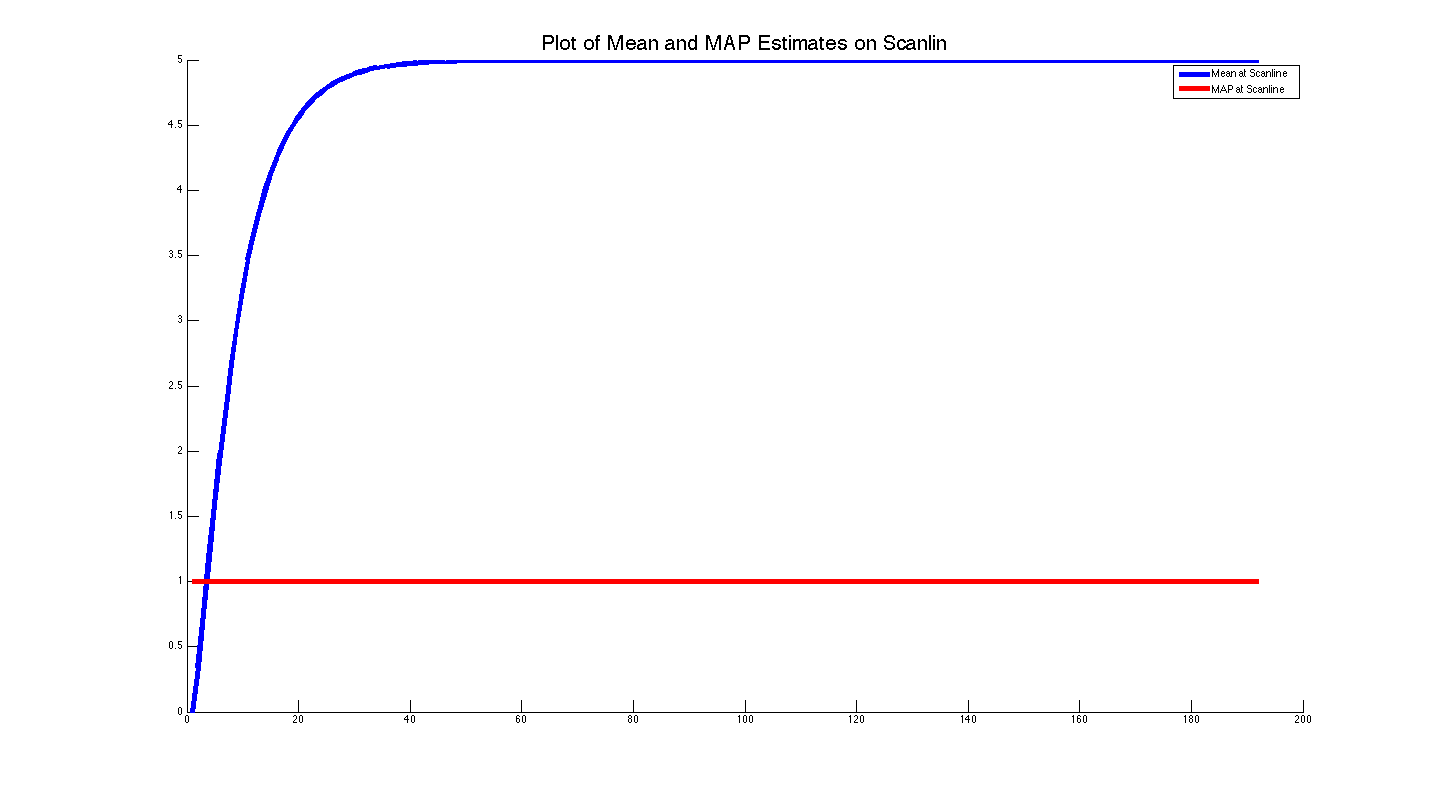
\includegraphics[scale=.18]{5_1lambda0_b}
    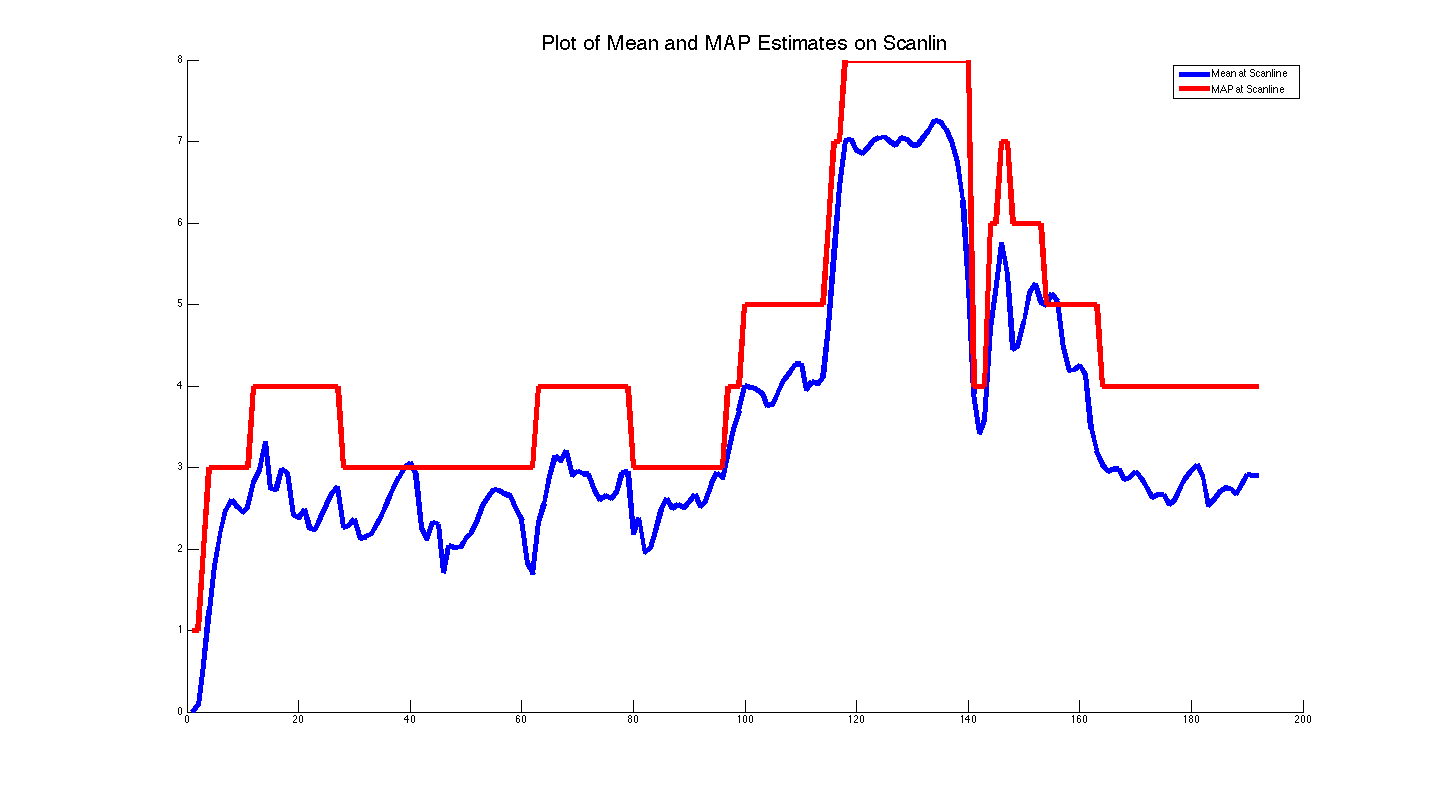
\includegraphics[scale=.18]{5_1lambda1_b} \newline

    \hspace{-40pt}
    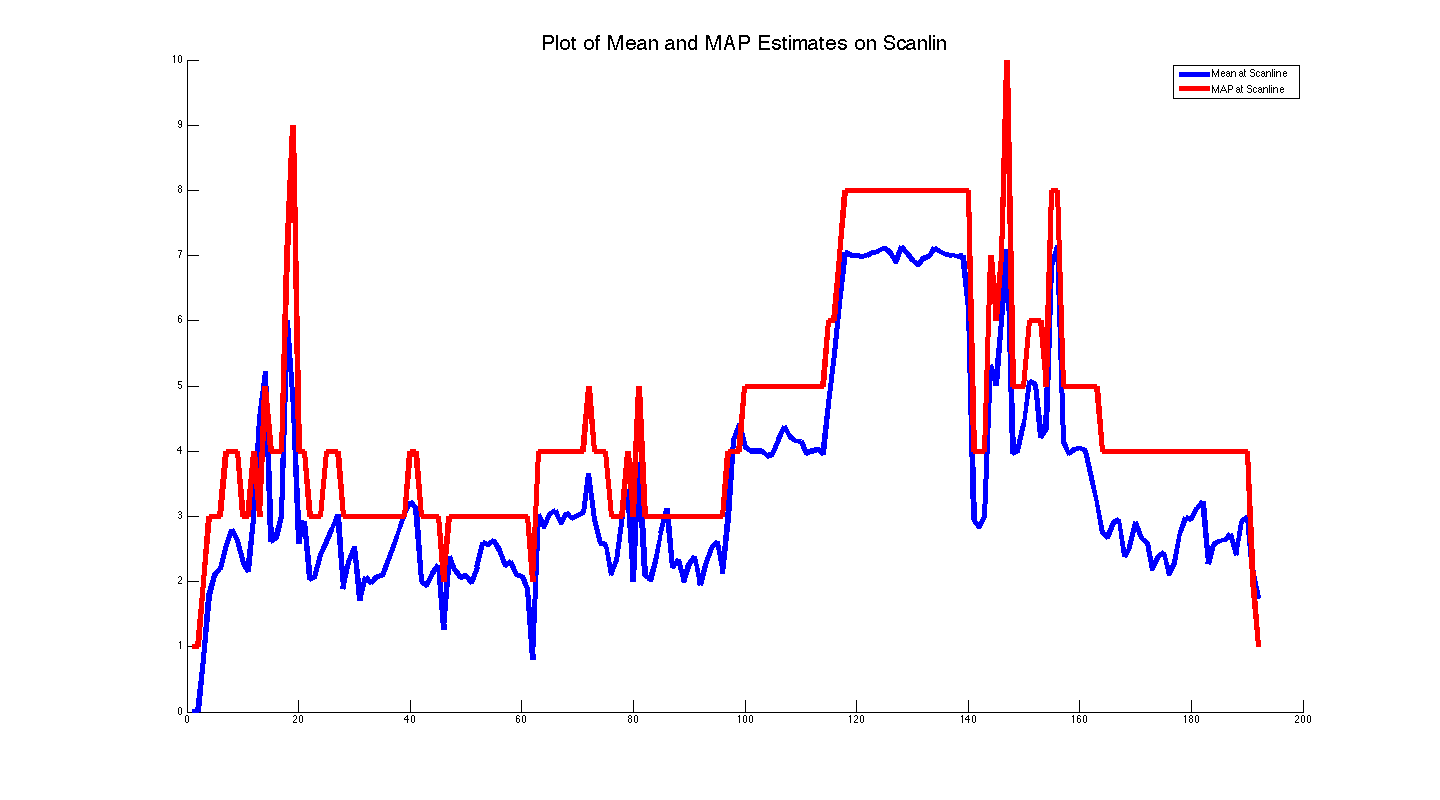
\includegraphics[scale=.18]{5_1lambda5_b}
    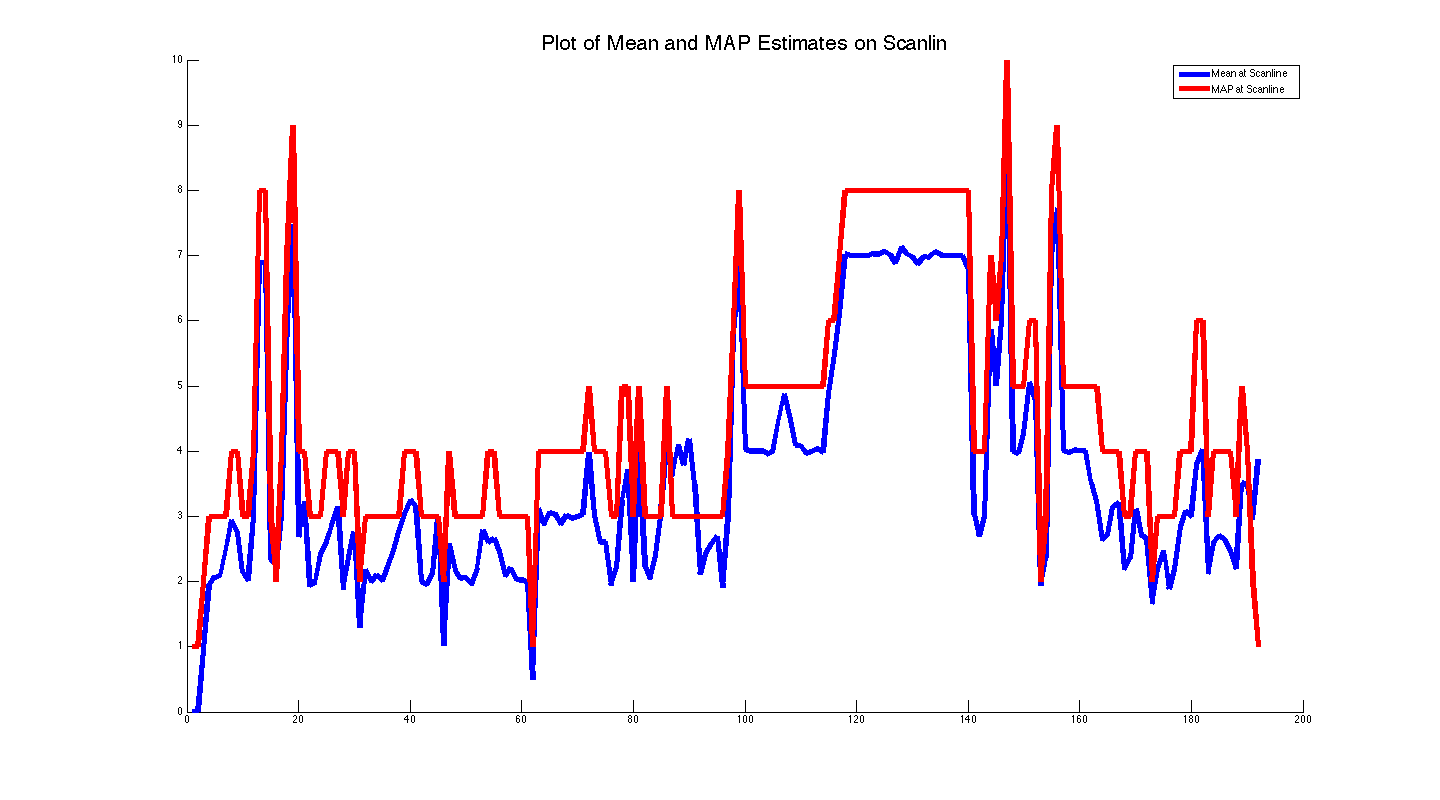
\includegraphics[scale=.18]{5_1lambdaOne_b} \newline

The top two plots show that decreasing $\lambda$ generates a more uniform mean estimate to the disparity, where as the bottom two plots show that increasing $\lambda$ generates a mean estimate that has more spikes and less uniform.  This is because $\lambda$ determines the weight we place on the difference in disparities.  The higher $\lambda$, the stronger the weights are applied, and therefore the more likley the results vary.
\newline

\textbf{(I)} Mean and MAP disparity as an image:  
\newline

\hspace{-70pt}
\DeclareGraphicsExtensions{.pdf,.png,.jpg}
    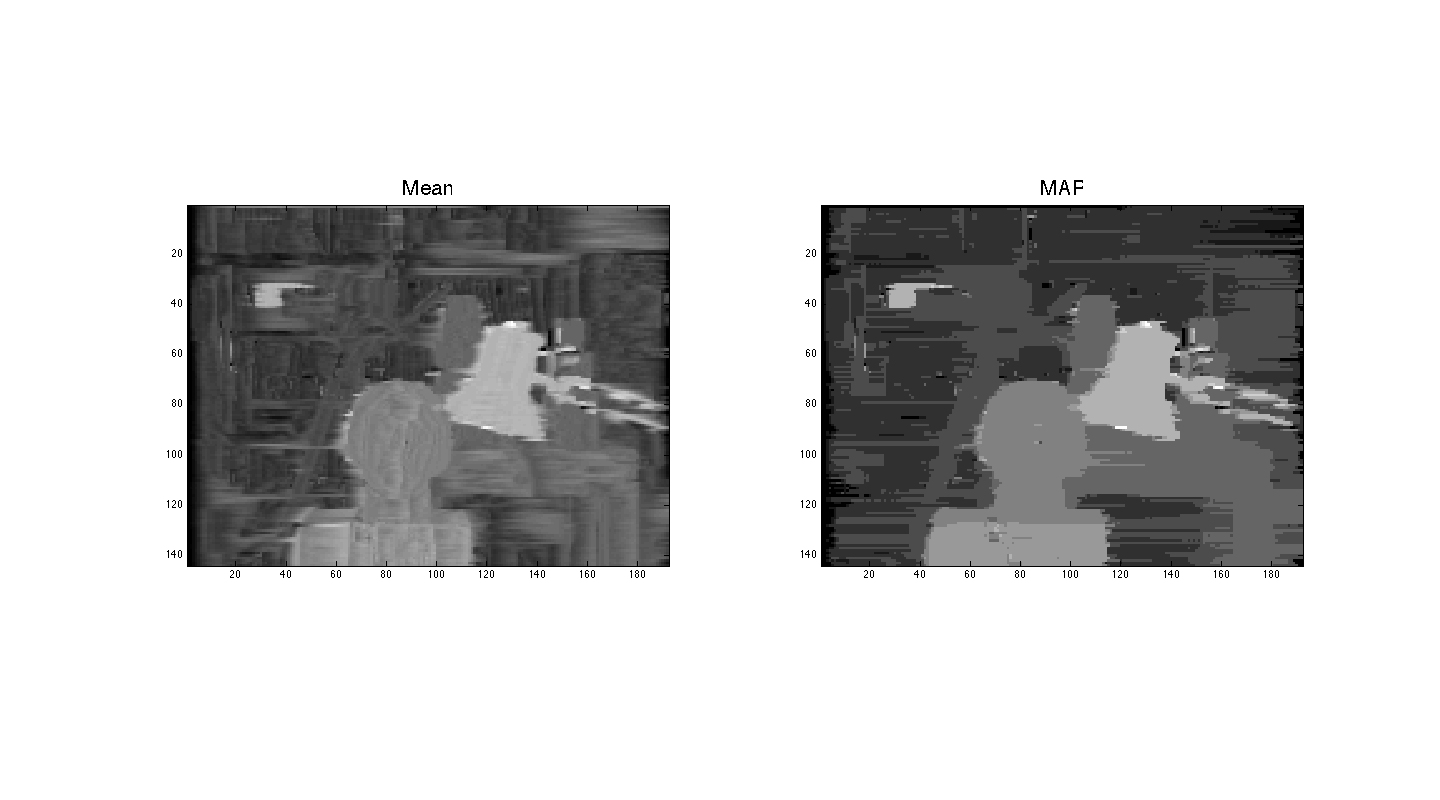
\includegraphics[scale=.4]{5_1g}

\textbf{(J)} Calculating the MAP estimate required an update to the message update equation.  Instead of doing a sum, do a max operation:  
\newline

\begin{center}
$m_{p \to q}(x_q) = max_{x_p} \phi(x_p) \psi(x_p, x_q) \prod\limits_{s \in \eta{p}/q} m_{s \to p}(x)$
\end{center}

Then computing the MAP estimate is the \texttt{arg\_max} index out of the largest marginal probabilities, given you the disparity that produces the max marginal.  From part G, we see that there is a difference bewteen the Mean and MAP estimates.  The MAP estimate tends to have a higher average and more smooth compared to the Mean estimate.  Also, the MAP is more step-like where as the Mean is more sporadic.
\newline

\textbf{Visualization:} For convenience, this is a complete small version of the ouput for \texttt{Prob1.m}
\newline

\DeclareGraphicsExtensions{.pdf,.png,.jpg}
    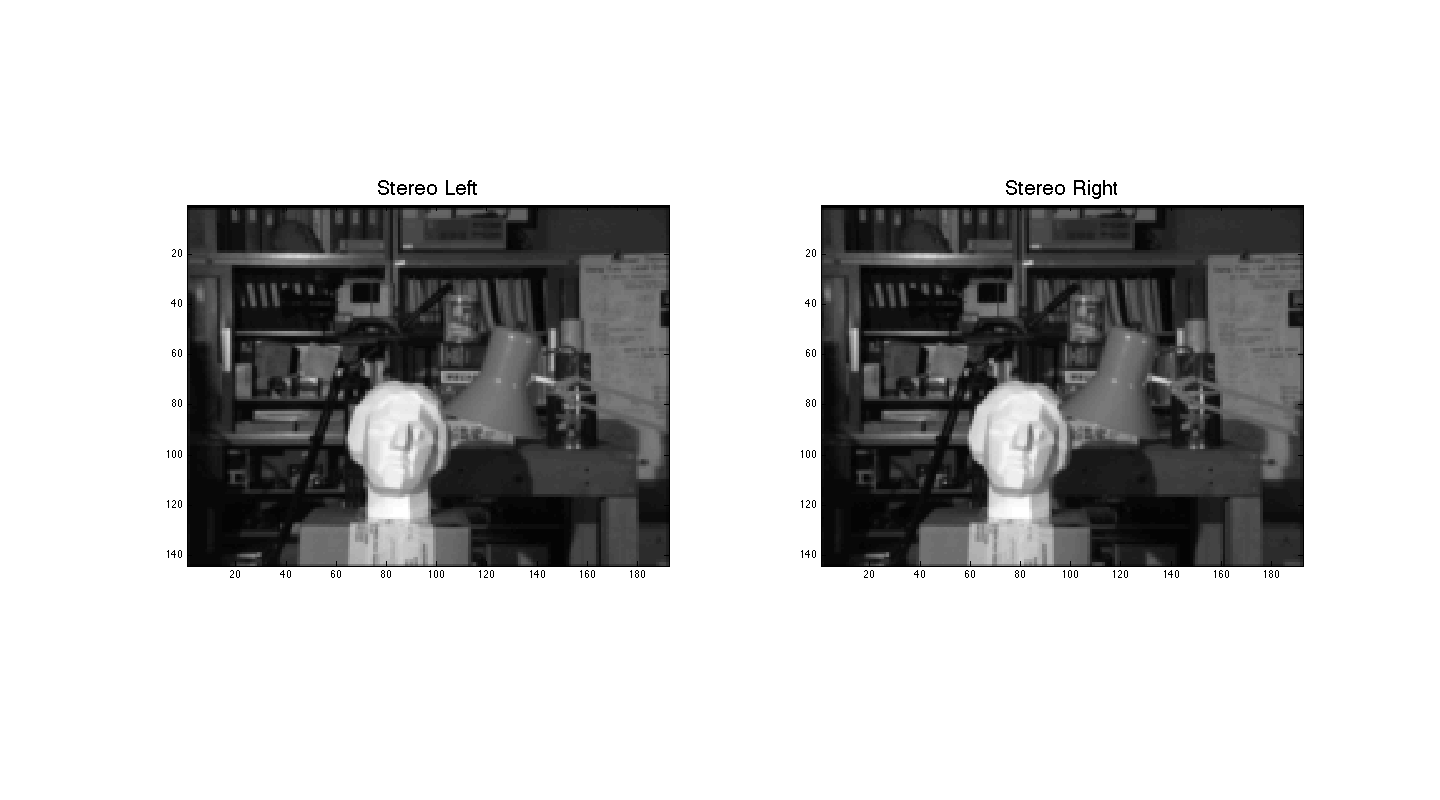
\includegraphics[scale=.15]{5_1a}
    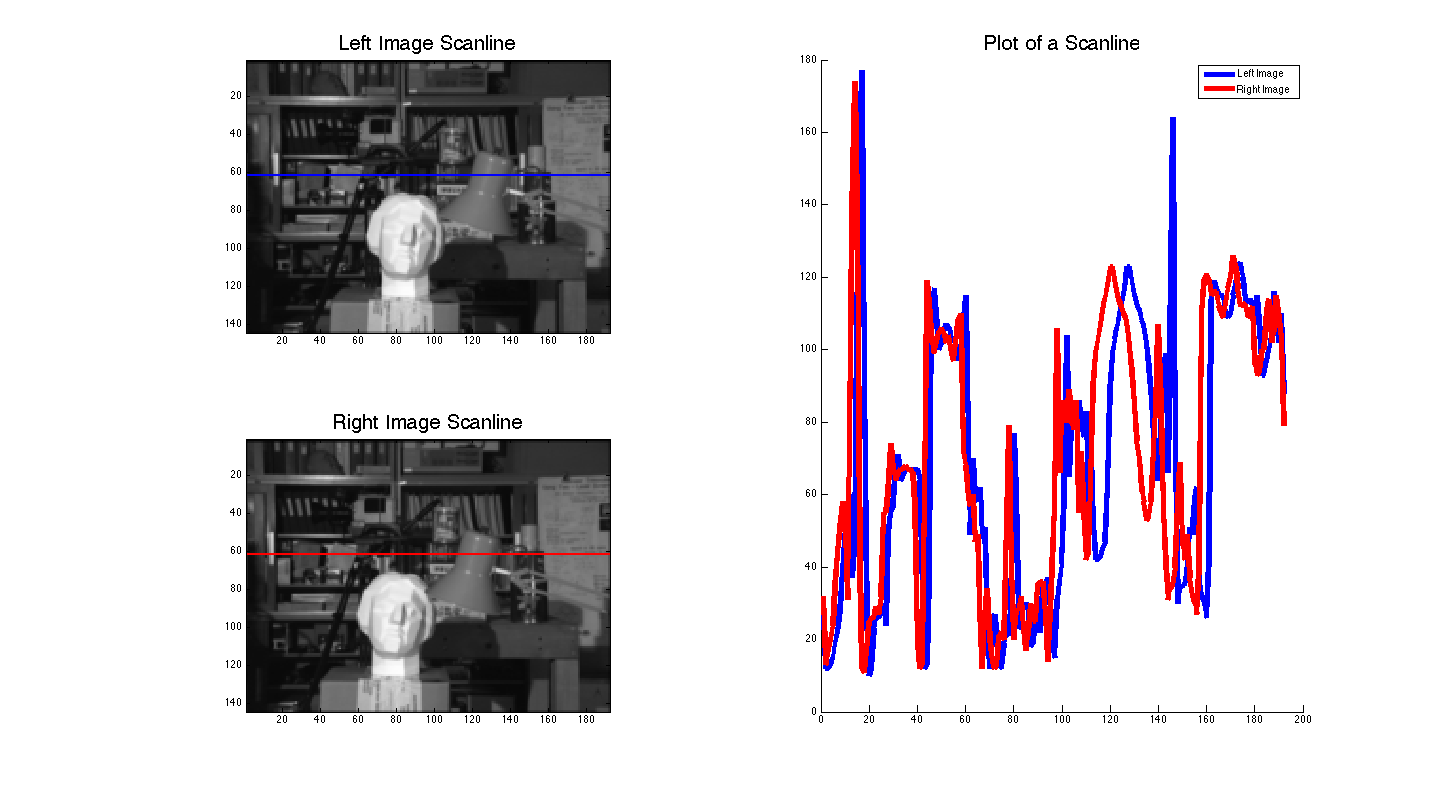
\includegraphics[scale=.15]{5_1b} \newline
    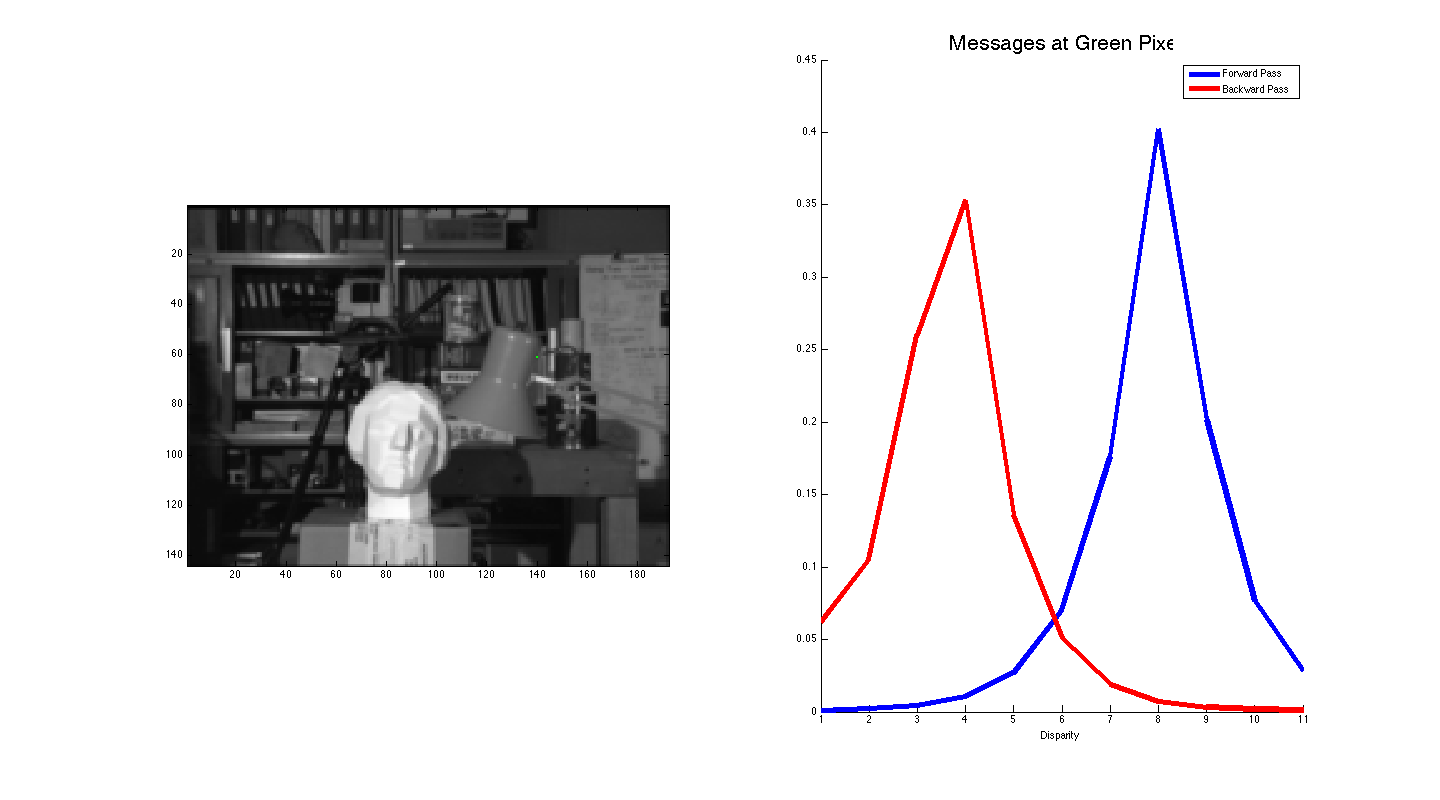
\includegraphics[scale=.15]{5_1c}
    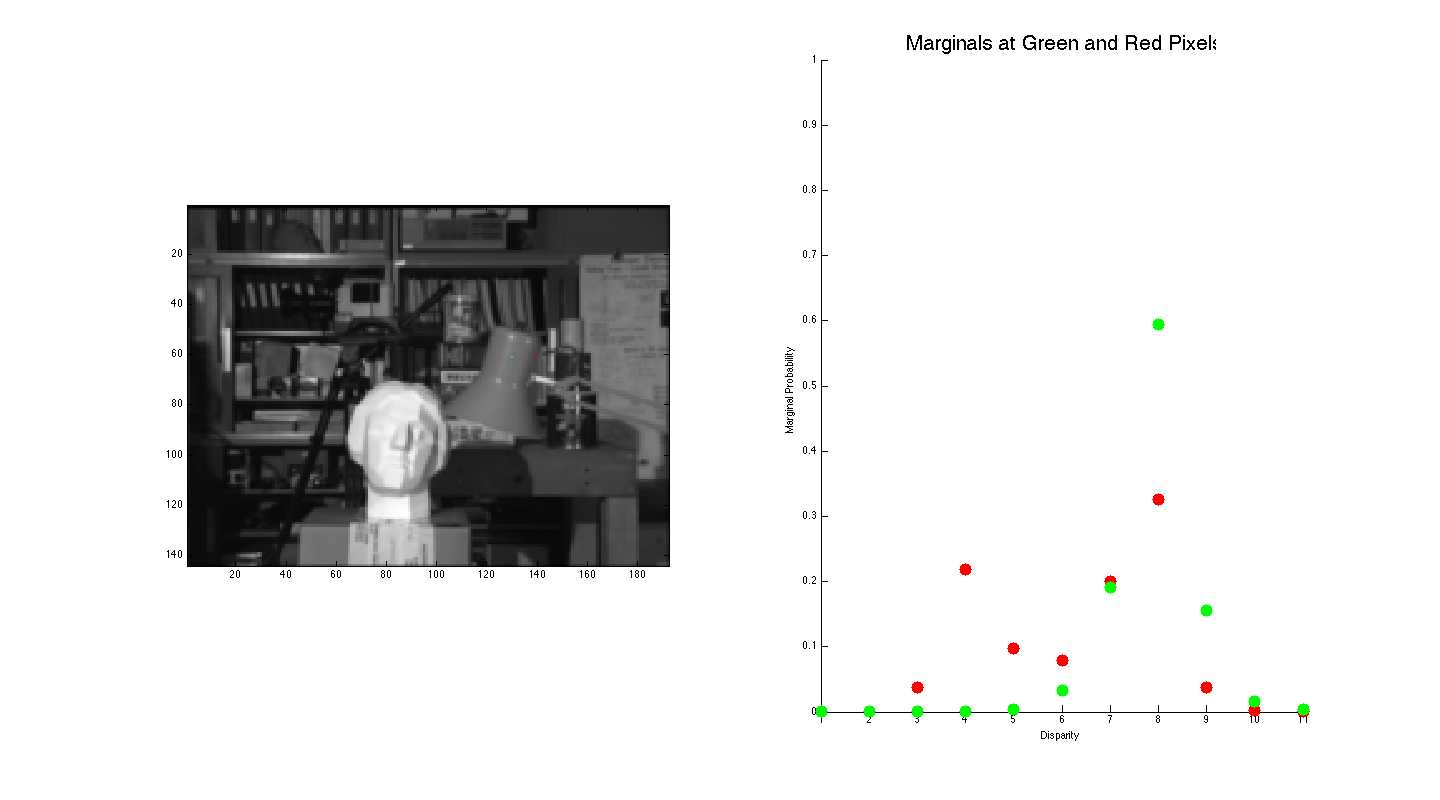
\includegraphics[scale=.15]{5_1d} \newline
    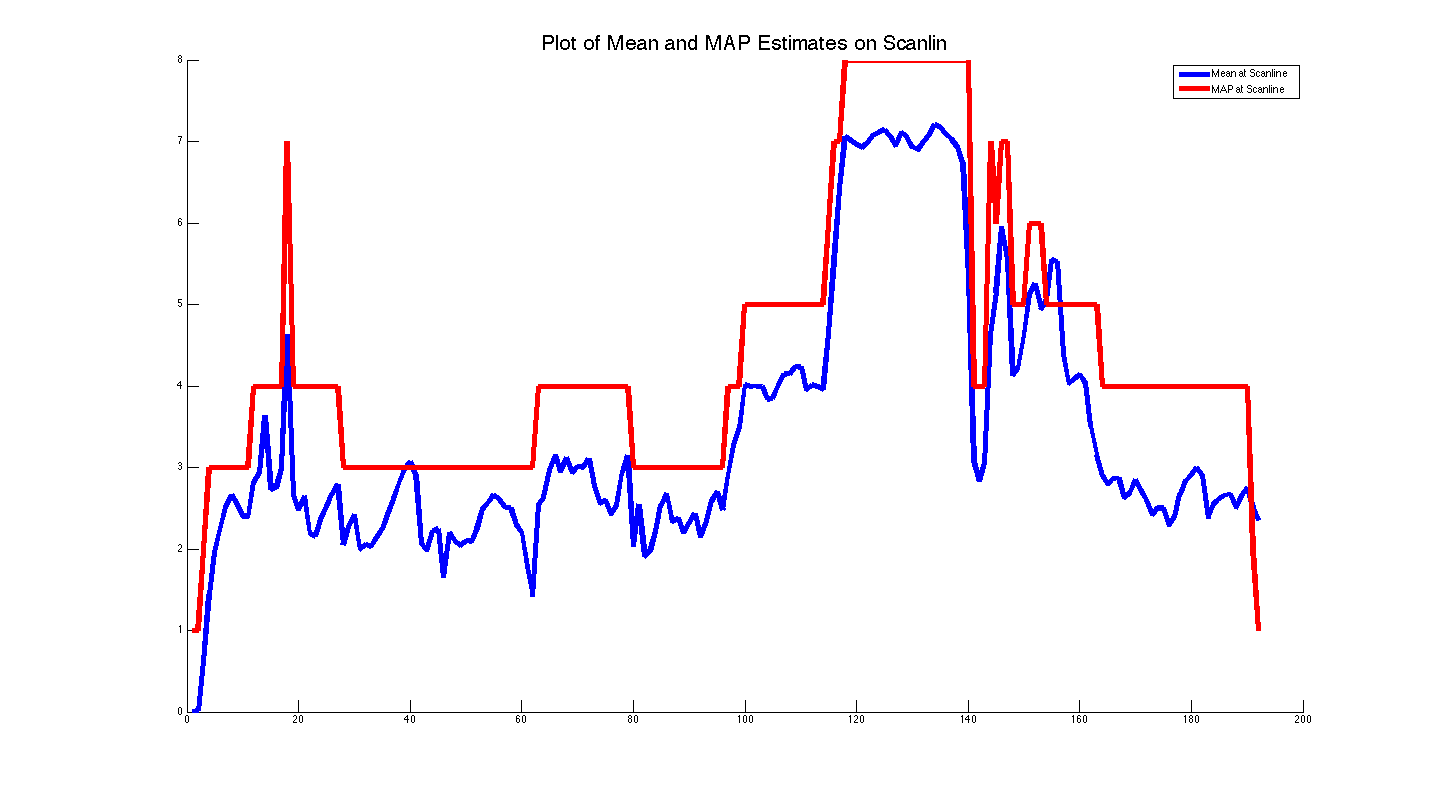
\includegraphics[scale=.15]{5_1e}
    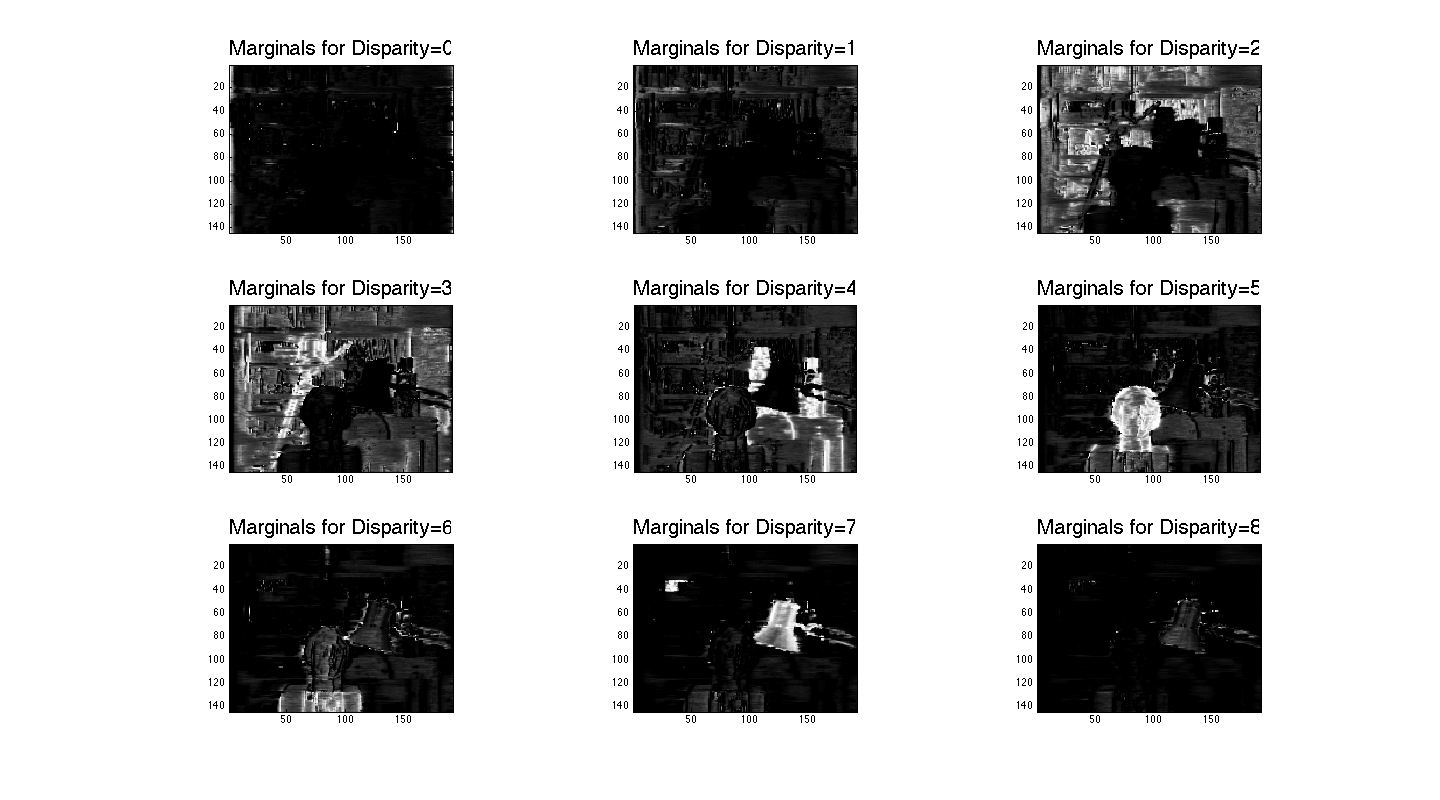
\includegraphics[scale=.15]{5_1f} \newline
    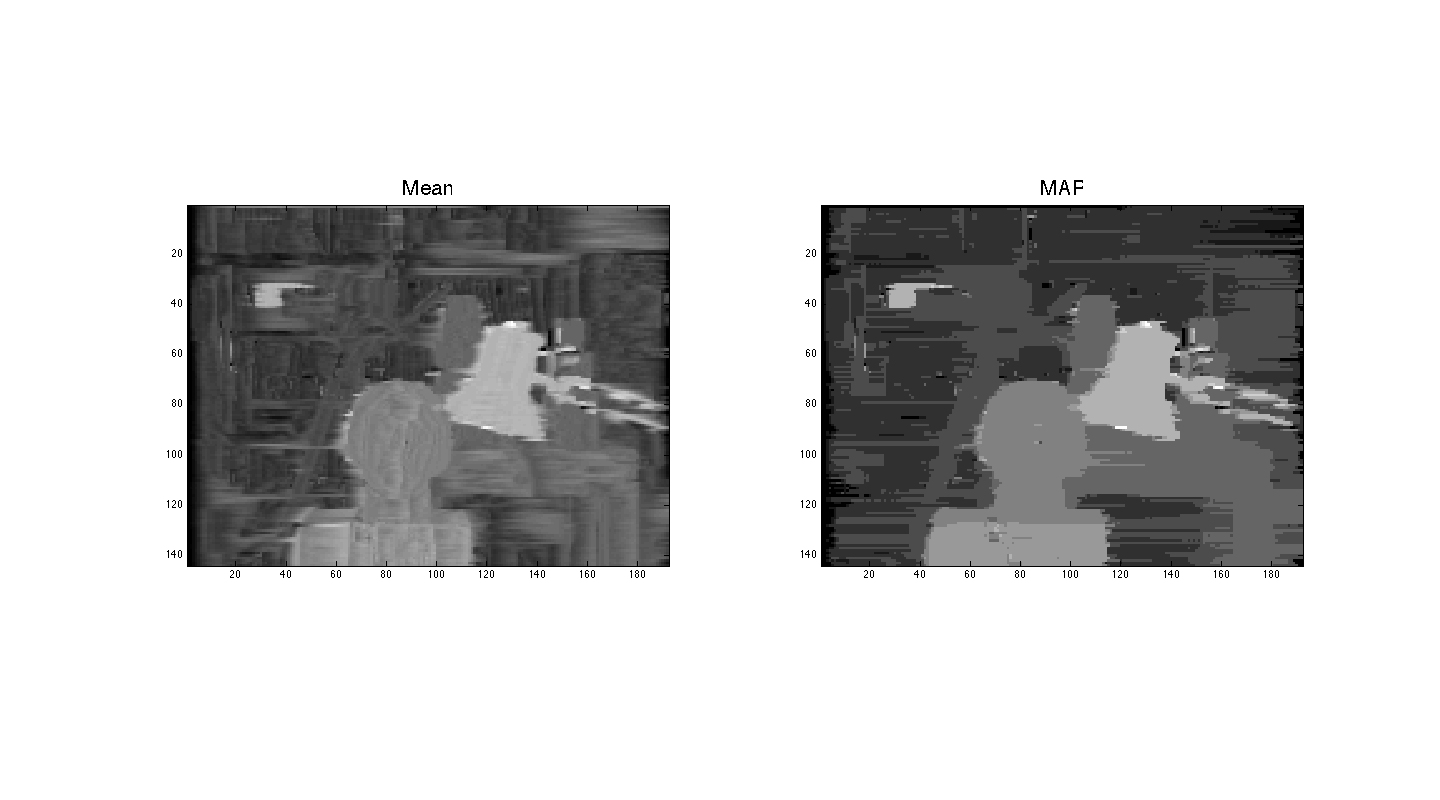
\includegraphics[scale=.15]{5_1g}


\section*{Problem 5.2}
\tabT In this problem, I implemented the Efros and Leung algorithm for texture synthesis.  I followed pseudocode provided at \texttt{http://graphics.cs.cmu.edu/people/efros/research/NPS/alg.html}.  It is repeated below for convenience.
\newline

\texttt{
function GrowImage(SampleImage,Image,WindowSize) \newline
\tabT\tabT  while Image not filled do\newline
\tabT\tabT\tabT    progress = 0\newline
\tabT\tabT\tabT    PixelList = GetUnfilledNeighbors(Image)\newline
\tabT\tabT\tabT    foreach Pixel in PixelList do\newline
\tabT\tabT\tabT\tabT     Template = GetNeighborhoodWindow(Pixel)\newline
\tabT\tabT\tabT\tabT     BestMatches = FindMatches(Template, SampleImage)\newline
\tabT\tabT\tabT\tabT     BestMatch = RandomPick(BestMatches)\newline
\tabT\tabT\tabT\tabT     if (BestMatch.error < MaxErrThreshold) then\newline
\tabT\tabT\tabT\tabT\tabT      Pixel.value = BestMatch.value\newline
\tabT\tabT\tabT\tabT\tabT     progress = 1\newline
\tabT\tabT\tabT\tabT    end\newline
\tabT\tabT\tabT   end\newline
\tabT\tabT\tabT   if progress == 0 \newline
\tabT\tabT\tabT\tabT    then MaxErrThreshold = MaxErrThreshold * 1.1\newline
\tabT\tabT end\newline
\tabT\tabT return Image\newline
\tabT end\newline
}
\newline

Although I have a slightly different implementation, the two main functions that was needed to be constructed was \texttt{SynthTexture} and a subroutine called \texttt{FindMatches}.
\newline

\begin{center}
\hspace{100pt}
\DeclareGraphicsExtensions{.pdf,.png,.jpg}
    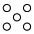
\includegraphics[scale=1, trim = 0pt 0pt 0pt 0pt, clip]{rings}\newline
\end{center}

Below are the results of running the texture \texttt{rings.jpg} (shown above) using window widths $w=5,7,13, s = [100,100]$ and an initial starting seed of $(x,y) = (4,32)$.

\DeclareGraphicsExtensions{.pdf,.png,.jpg}
	\hspace{-70pt}
    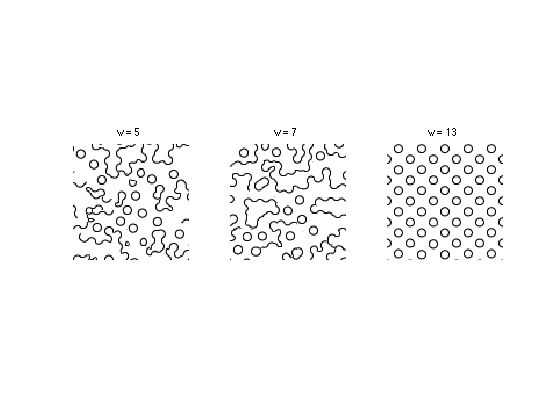
\includegraphics[scale=1, trim = 0pt 150pt 0pt 100pt, clip]{5_2a}\newline

Here we see that the performance increases as the window size gets larger.  When $w = 13$, the texture looks like the original.  For smaller window sizes, only few of the dots are formed.  Below shows the results iterating over a particular window size with the same starting seed. 

	\hspace{-20pt}
    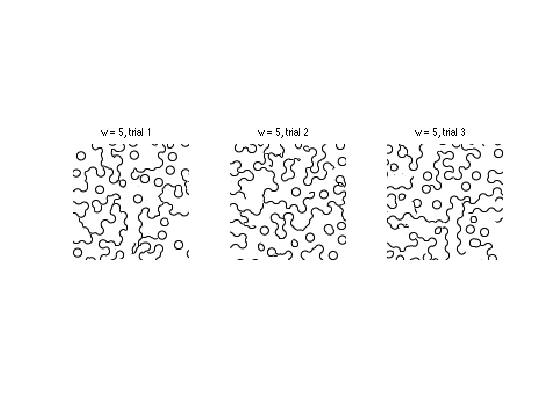
\includegraphics[scale=1, trim = 60pt 150pt 0pt 100pt, clip]{5_2b}\newline
    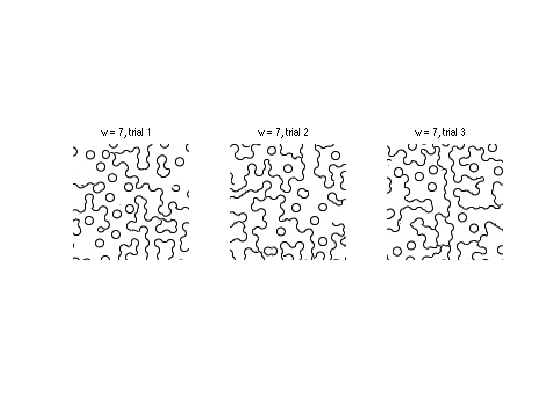
\includegraphics[scale=1, trim = 60pt 150pt 0pt 100pt, clip]{5_2c}\newline
    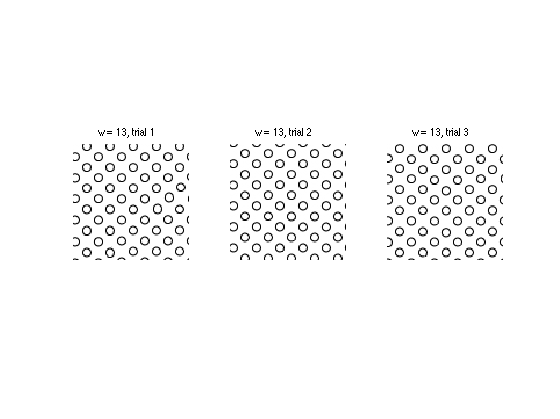
\includegraphics[scale=1, trim = 60pt 150pt 0pt 100pt, clip]{5_2d}\newline

We see for the smaller window sizes, running the algorithm multiple times with the same starting seeds had different results, this is because as the texture is getting generated, the source texture is contstantly estimating each pixel based on the prior estimated pixel.  Therefore, as the algorithm is incrementally adding pixels, it has to decide whether to complete an edge or not.  Since the window size is smaller, the adjusted rings texture has edges on the borders.  On the otherhand, the results for $w=13$ look similar.  Perhaps this is because the window is large enough that it can be repeated based on the borders of the original source texture and not estimating whether to continue/end on edge of a ring. 















\end{document}
